\documentclass[letterpaper]{article}
\usepackage[margin=1in]{geometry}
\usepackage[utf8]{inputenc}
\usepackage{textcomp}
\usepackage{amssymb}
\usepackage{natbib}
\usepackage{graphicx}
\usepackage{gensymb}
\usepackage{amsthm, amsmath, mathtools}
\usepackage[dvipsnames]{xcolor}
\usepackage{enumerate}
\usepackage{mdframed}
\usepackage[most]{tcolorbox}
\usepackage{csquotes}
% https://tex.stackexchange.com/questions/13506/how-to-continue-the-framed-text-box-on-multiple-pages

\tcbuselibrary{theorems}

\newcommand{\R}{\mathbb{R}}
\newcommand{\Z}{\mathbb{Z}}
\newcommand{\N}{\mathbb{N}}
\newcommand{\Q}{\mathbb{Q}}
\newcommand{\C}{\mathbb{C}}
\newcommand{\code}[1]{\texttt{#1}}
\newcommand{\mdiamond}{$\diamondsuit$}
\newcommand{\PowerSet}{\mathcal{P}}
\newcommand{\Mod}[1]{\ (\mathrm{mod}\ #1)}
\DeclareMathOperator{\lcm}{lcm}

%\newtheorem*{theorem}{Theorem}
%\newtheorem*{definition}{Definition}
%\newtheorem*{corollary}{Corollary}
%\newtheorem*{lemma}{Lemma}
\newtheorem*{proposition}{Proposition}


\newtcbtheorem[number within=section]{theorem}{Theorem}
{colback=green!5,colframe=green!35!black,fonttitle=\bfseries}{th}

\newtcbtheorem[number within=section]{definition}{Definition}
{colback=blue!5,colframe=blue!35!black,fonttitle=\bfseries}{def}

\newtcbtheorem[number within=section]{corollary}{Corollary}
{colback=yellow!5,colframe=yellow!35!black,fonttitle=\bfseries}{cor}

\newtcbtheorem[number within=section]{lemma}{Lemma}
{colback=red!5,colframe=red!35!black,fonttitle=\bfseries}{lem}

\newtcbtheorem[number within=section]{example}{Example}
{colback=white!5,colframe=white!35!black,fonttitle=\bfseries}{def}

\newtcbtheorem[number within=section]{note}{Important Note}{
        enhanced,
        sharp corners,
        attach boxed title to top left={
            xshift=-1mm,
            yshift=-5mm,
            yshifttext=-1mm
        },
        top=1.5em,
        colback=white,
        colframe=black,
        fonttitle=\bfseries,
        boxed title style={
            sharp corners,
            size=small,
            colback=red!75!black,
            colframe=red!75!black,
        } 
    }{impnote}
\usepackage[utf8]{inputenc}
\usepackage[english]{babel}
\usepackage{fancyhdr}
\usepackage[hidelinks]{hyperref}

\pagestyle{fancy}
\fancyhf{}
\rhead{CSE 101}
\chead{Wednesday, February 2, 2022}
\lhead{Lecture 12}
\rfoot{\thepage}

\setlength{\parindent}{0pt}

\begin{document}

\section{Searching Problem}
Given a sorted list $L$ and a number $x$, find the location of $x \in L$.

\subsection{Naive Algorithm}
The naive algorithm is to iterate over each element in $L$ and see where $x$ is in $L$. This takes $\BigO(n)$ time as the element in question might be at the end of the list.  

\bigskip 

\textbf{Remark:} Usually, you cannot beat $\BigO(n)$ because any algorithm needs to read the entire input. \emph{However}, since the list is guaranteed to be sorted, we can do better.

\subsection{Algorithm Idea}
First, we want to split $L$ into two sublists. The idea is to take advantage of the fact that $L$ is sorted to see which of the two sublists we should check. Essentially:
\begin{itemize}
    \item If $L[i] > x$, then the location must be before $i$.
    \item If $L[i] < x$, then the location must be after $i$. 
    \item If $L[i] = x$, then we found it. 
\end{itemize}
Of course, we don't want to actually \emph{split} the list; that would take too much time. Instead, we can have two indices $i$ and $j$ which determine which part of the list to check. 

\subsection{Divide and Conquer Algorithm}
\begin{verbatim}
    // Search between L[i] and L[j]
    BinarySearch(L, i, j, x)
        // This is the base case. 
        if j < i
            return 'error'
        k = (i + j) / 2
        if L[k] == x
            return k
        if L[k] > x
            return BinarySearch(L, i, k - 1, x)
        if L[k] < x 
            return BinarySearch(L, k + 1, j, x)
\end{verbatim}
To analyze the runtime, we note the following:
\begin{itemize}
    \item \underline{Base Case:} The base case runs in $\BigO(1)$ time; this is obvious (and is expected for any base case).
    \item \underline{Divide \& Conquer:} The divide and conquer part comes in several steps. 
    \begin{itemize}
        \item \underline{Divide:} The divide part comes from the calculation of $k$, which determines what range we want to consider when recursively calling \code{BinarySearch}.
        \item \underline{Conquer:} We're only interested in running through a \emph{subset} of $L$. Recall that, with binary search, while we're still working with the big list $L$, the range that we check will always be half of the previous range that was considered. With this in mind, it takes $T(n / 2 + \BigO(1))$ time to recursively solve one subproblem of size $\frac{n}{2}$. The $\BigO(1)$ is due to the possibility that one of the two ranges may have unequal sizes (e.g. one range covers 5 elements and another range has covers 6). At the end of the day, we can just simplify this down to $T(n / 2)$. 
        \item \underline{Combine:} Combining the answer is as simple as returning $k$. 
    \end{itemize}
\end{itemize}
We then have (by the Master Theorem):
\[T(n) = T(n / 2) + \BigO(n)\]
Note that $a = 1$, $b = 2$, and $d = 0$, so the final runtime is given by the Master Theorem:
\[\BigO(\log n)\]


\subsection{Puzzles \& Applications}
\begin{mdframed}[]
    Binary search, or something related to that, occurs when we try to solve a problem with a finite number of possible answers and, every time we make a guess as to what the answer is, we eliminate a \emph{constant fraction} of the possibilities. \textbf{Put it another way}, lots of puzzles have binary search-like answers; as long as you can spend \emph{constant time} to divide your search space by some constant fraction, you can use binary search in $\BigO(\log(n))$ time.  
\end{mdframed}
Suppose you have 27 coins, one of which is \emph{heavier} than the others, and a balance. You are asked to determine the heavy coins in 3 weighings. The idea is: 
\begin{itemize}
    \item After one weighing, you're down to 9 possibilities. 
    \item After another weighing, you're down to 3 possibilities.
    \item After a third weighing, you're down to just 1 possibility. 
\end{itemize}







\section{Closest Pair of Points}
Given $n$ points in the plane, $(x_1, y_1), \dots, (x_n, y_n)$, find the pair $(x_i, y_i)$ and $(x_j, y_j)$ whose Euclidean distance is as small as possible. 

\subsection{Naive Algorithm}
The naive algorithm is to simply try every pair of points. This runs in $\BigO(n^2)$ time; you have $n$ points so $n^2$ possibilities. 

\subsection{Divide and Conquer Outline}
In order to use divide and conquer, you need to find some way to divide the set of points into two equally sized subsets. One reasonable way to do this is to draw a line and cut the plane so that you can consider the points on the left and right of the line. 
\begin{center}
    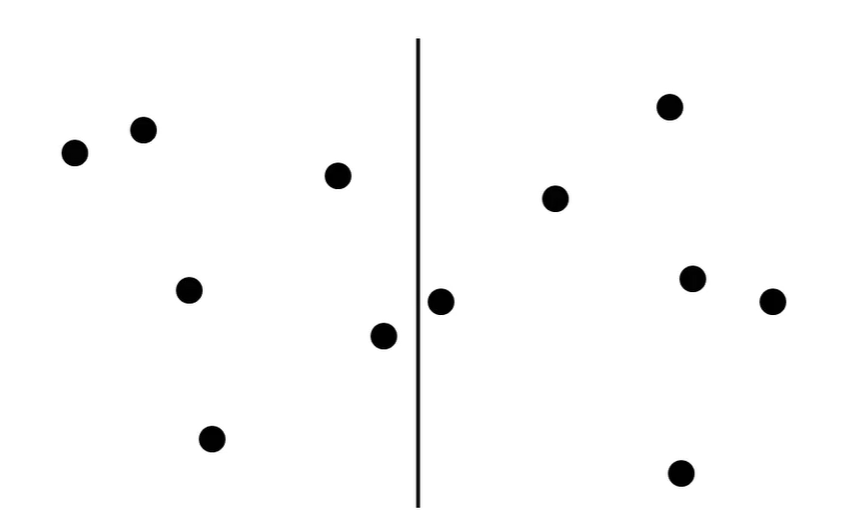
\includegraphics[scale=0.2]{../assets/closest_pts_1.png}
\end{center}
From there, you can compute the closest pair of points on each side. 
\begin{center}
    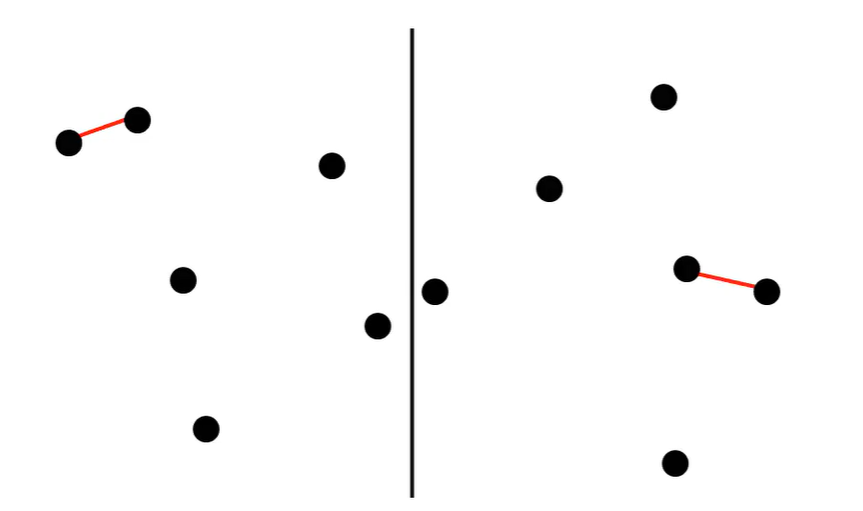
\includegraphics[scale=0.2]{../assets/closest_pts_2.png}
\end{center}
After we do this, we need to somehow recombine the answers to our subproblems so we can get the answer. \textbf{However}, we can't simply just return the better of the two pairs (denoted by the red line) because it's possible that the best pair of points actually \emph{crosses} the line that we used to cut our problem in half (which we didn't consider since these two points are in separate subsets). So, what do we do? 

\subsubsection{Observation}
Consider the following set of points, with the dividing line: 
\begin{center}
    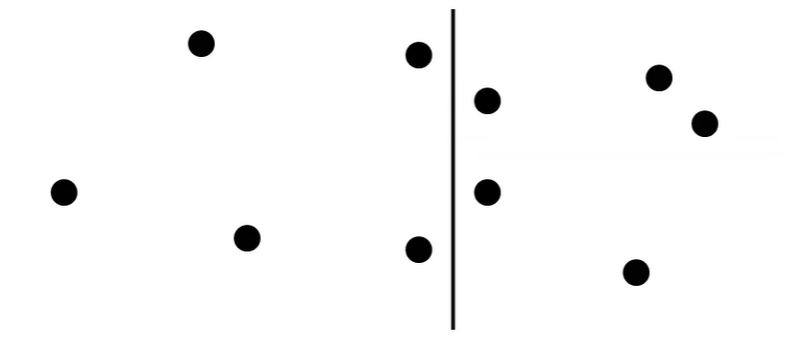
\includegraphics[scale=0.3]{../assets/closest_pts_3.png}
\end{center}
Suppose that the closest pair of points on \emph{either side} of the dividing line is at distance $\delta$; that is, two points on the same side has distance $\delta$. 
\begin{center}
    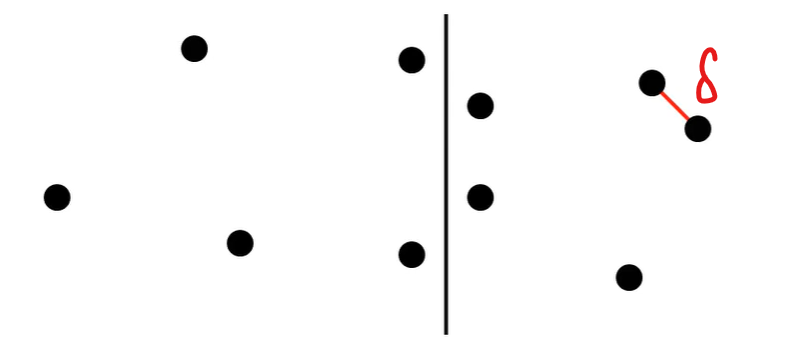
\includegraphics[scale=0.3]{../assets/closest_pts_4.png}
\end{center}
At the very least, we only need to care about points \emph{within} $\delta$ of the dividing line. So, we only need to consider a \emph{strip} of width $2\delta$:
\begin{center}
    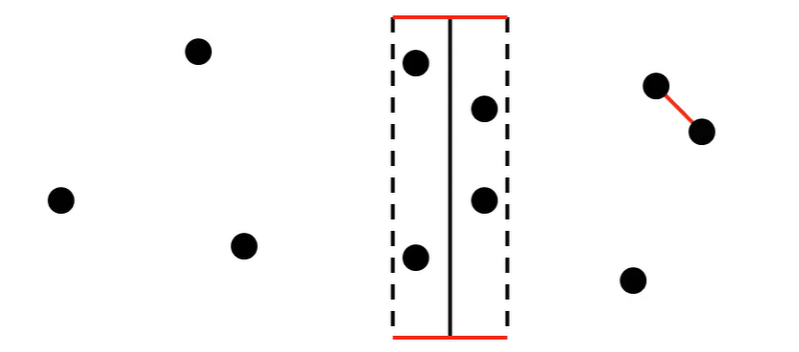
\includegraphics[scale=0.3]{../assets/closest_pts_5.png}
\end{center}
In our case here, we now only focus our attention on any points within this strip. We now need to know if there is some pair of points in this strip where the distance between the points in that pair is \emph{less than} $\delta$. In other words, is there a pair of points in this strip whose distance is \emph{better} than the distance that we already found (i.e. $\delta$)?


\subsubsection{Main Idea}
The main idea is that we know that any pair of points on the same side of the line has to be separated by at least $\delta$. So, the points inside this strip must be reasonably spaced out vertically. So, if we want to find some pair of points that are closer to $\delta$, there can't be that many other points in between them. If we sort the points vertically (by their $y$-coordinates), then two points that are super close to each other cannot be far off in that ordering. 
\begin{proposition}
    Take the points within $\delta$ of the dividing line and sort them by $y$-coordinate. Any one of these points can only be within $\delta$ of the 8 closest points on either side of it. 
\end{proposition}
So, sort everything by $y$-coordinate. Then, look at the next 8 points\footnote{What really matters is that this is \textbf{some constant}; it can be 5 or 10 or 127 or whatever.} in $y$-coordinate above it and the next 8 points in $y$-coordinate below it. Those are the only possible points that can possibly be within $\delta$ of the point that we're considering. 

\bigskip 

If the proposition is true, then this means we only need to check a few pair of points crossing the line. The \emph{idea} is that the points on each side of the line are separated by at least $\delta$. This is because we know that $\delta$ is the distance to the closest pair of points for any pair of points on either side of the line. This means that there isn't enough room to cram many points into a narrow region because this forces points to be spread out. 

\begin{mdframed}[]
    \begin{proof}
        Suppose we have the dividing line, some $\delta$, and a point.
        \begin{center}
            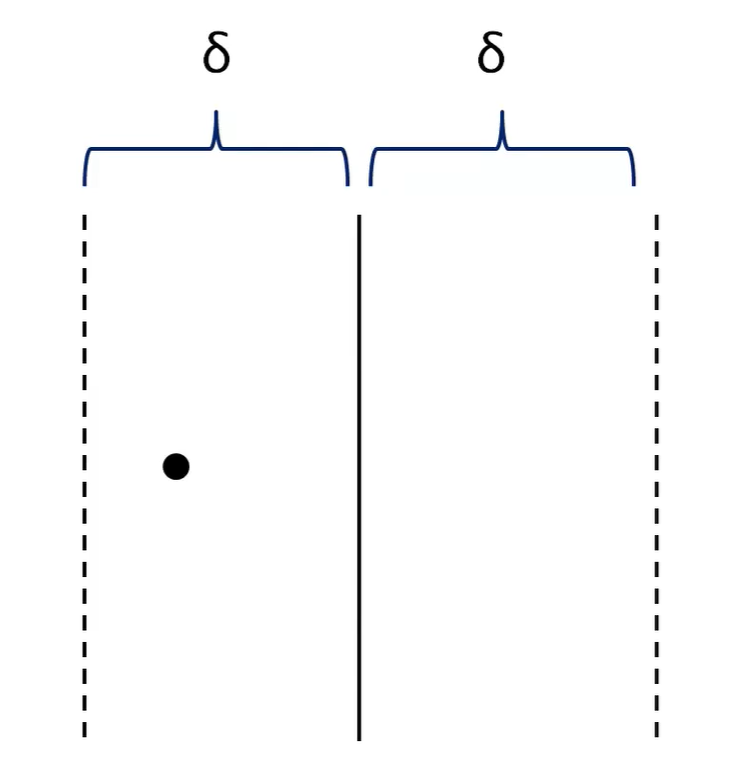
\includegraphics[scale=0.37]{../assets/closest_proof_1.png}
        \end{center}
        Any nearby point has to be within this strip and the $y$-coordinate of that point we're looking for must be within $\delta$ of the $y$-coordinate that we have. So, we can create a bigger box and every other point that we want to match this one point with must be somewhere in this box.
        \begin{center}
            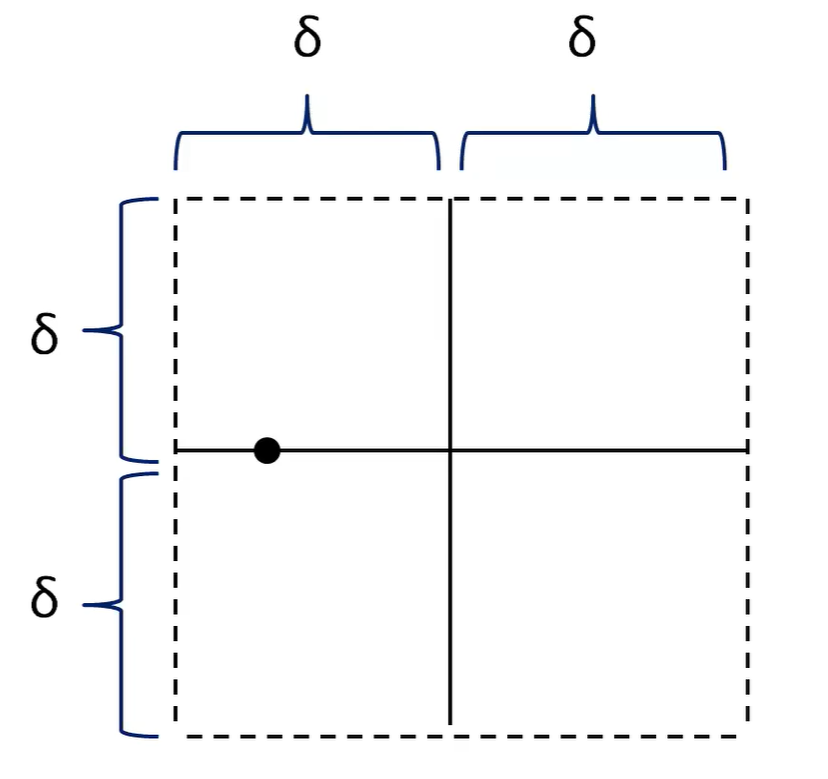
\includegraphics[scale=0.37]{../assets/closest_proof_2.png}
        \end{center}
        So, we can subdivide this region into $\delta / 2$-sided squares. 
        \begin{center}
            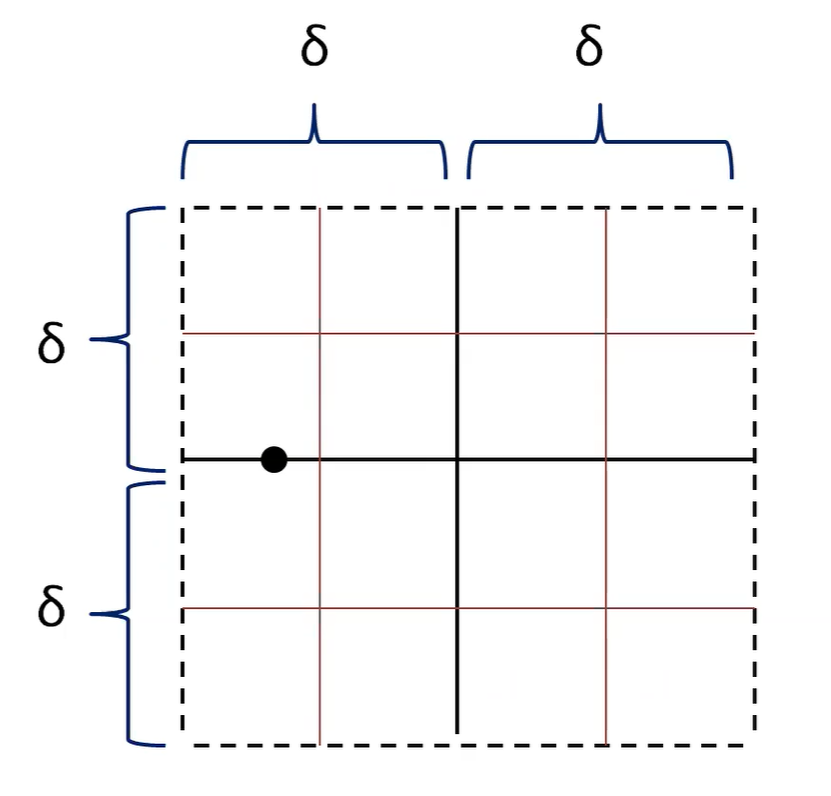
\includegraphics[scale=0.37]{../assets/closest_proof_3.png}
        \end{center}
        There are now 16 squares; 8 of them are above the point and 8 of them are below the point. The claim is that each of these little squares can have at most one point. This is because if we take any two points inside the same square, the distance between those points will be less than $\delta$. In particular, since every square is either on the left or right side of the dividing line, we can't have two points in the same square with distance less than $\delta$ because then there would be points on the same side of the dividing line with distance less than $\delta$. 
        \begin{center}
            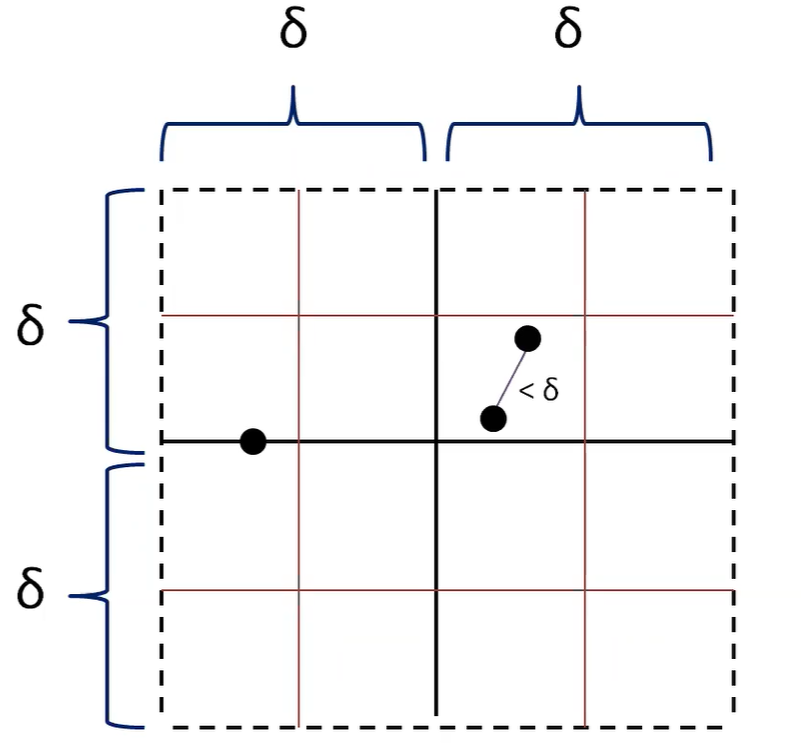
\includegraphics[scale=0.37]{../assets/closest_proof_4.png}

            \textbf{Figure:} Two points in the same square with distance less than $\delta$, a contradiction to our original claim that $\delta$ was the smallest distance between two points on the same side of the line. 
        \end{center}
        
        So, the point is that there is at most one point in each square\footnote{Note that there is a possibility that there is a point on the dividing line. In this case, just move the dividing line until there are no points on it. Alternatively, we can treat points on the line as being on the left/right of the dividing line.}. Thus, there are at most 8 points below and above our given point; any other points close to our given point must be farther than $\delta$ or outside of the strip. This completes the proof. 
    \end{proof}
\end{mdframed}

\subsection{The Algorithm}
\begin{verbatim}
    CPP(S)
        // Base case, brute force it. 
        If len(S) <= 3
            return closest distance 
        
        Find line L evenly dividing points.                     // (a)
        Sort S into S_{left}, S_{right}                         // (b)
        // D is delta 
        let D = min(CPP(S_{left}), CPP(S_{right}))              // (c)
        let T be the points within D of L                       // (d)
        Sort T by y-coordinate                                  // (d)
        Compare each element of T to 8 closest on either side.  // (e)
            Let min dist be D' 
        Return min(D, D')
\end{verbatim}

The runtime analysis is as follows: 
\begin{enumerate}[\hspace{0.5cm}(a)]
    \item First, finding the line that evenly divides the points take $\BigO(n)$ time. 
    \item Sorting the points into the two sets takes $\BigO(n)$ time. 
    \item The two recursive calls take $2T(n / 2)$ time. 
    \item Finding and sorting $T$ takes $\BigO(n\log(n))$ time. 
    \item Comparing each element of $T$ to 8 closest on either side takes $\BigO(n)$ time. 
\end{enumerate}
This gives us the recurrence: 
\[T(n) = \BigO(n\log(n)) + 2T(n / 2)\]
This is not a runtime recurrence that we can use the Master Theorem for; this is particularly because the Master Theorem uses $\BigO(n^d)$ whereas we have $\BigO(n\log(n))$. However, by running a Master Theorem-like argument, we have that 
\[T(n) = \BigO(n\log^{2}(n))\]
Alternatively, if we are more careful and have \code{CPP} take points already sorted by $y$-coordinate, we can reduce this runtime down to $\BigO(n\log(n))$. 

 
\end{document}